\documentclass[msc]{cls_bst/cls_file_ufam}

%nao mudar msc--- formato para mestrado
%compilar para GS
%CTRL+SHIFT+L
%CTRL+SHIFT+D
%CTRL+SHIFT+G

%compilar DVI (figuras em eps)
%%CTRL+SHIFT+X


%%%%%%%%%%%%%%%%%%%%%%%%%%%%%%%%%%%%%%%%%%%%%%%%%%%%%%%%%%
%% pacotes e sets

\usepackage{epstopdf}
\usepackage[latin1]{inputenc}
\usepackage[T1]{fontenc}
\usepackage[english,brazil]{babel}
\usepackage{indentfirst}
\usepackage{subfigure}
\usepackage{epsfig}
%\usepackage{booktabs}
\usepackage{cite}
\usepackage{longtable}
\usepackage{setspace}
\usepackage{rotating}
\usepackage{graphicx}
\usepackage{dsfont}
\usepackage{enumerate}
\usepackage{amsmath}
\usepackage{color}
\usepackage{bbm}
%\usepackage[portugues,algoruled,longend]{algorithm2e}
%\usepackage{algorithmic}
\usepackage{amssymb}
\usepackage{fancyhdr} %op1: boxed,lined %op2: ruled,vlined
%\usepackage[portugues,boxed,lined]{algorithm2e}
\setcounter{secnumdepth}{3}      % numeracao ate subsubsecao
\setcounter{tocdepth}{2}         % �ndice ate subsubsecao
\setcounter{chapter}{0}
\setlength{\parindent}{1.25cm}   % indenta��o de 1.25 cm

%\usepackage{upgreek}
\usepackage[final]{pdfpages}
%\usepackage[number=none]{glossary}
\usepackage{url}
\usepackage{float}
\usepackage{multirow,colortbl,array}
\usepackage{hhline}
%%%%%%%%%%%%%%%%%%%%%%%%%%%%%%%%%%%%%%%%%%%%%%%%%%%%%%%%%%

%\makeglossary
%\makelosymbols
%\makeloabbreviations

\begin{document}

\newcommand{\sgn}{\mathop{\mathrm{sgn}}}



%%%%%%%%%%%%%%%%%%%%%%%%%%%%%%%%%%%%%%%%%%%%%%%%%%%%%%%%%%

%% hyphenation
%\hyphenation{o-ri-gi-nal}
%\hyphenation{con-si-de-rar-mos}
%\hyphenation{re-co-nhe-ci-men-to}
%%%%%%%%%%%%%%%%%%%%%%%%%%%%%%%%%%%%%%%%%%%%%%%%%%%%%%%%%%



%%%%%%%%%%%%%%%%%%%%%%%%%%%%%%%%%%%%%%%%%%%%%%%%%%%%%%%%%%
%% capa

  %%%%%%%%%%%%%%%%%%%%%%%%%%%%%%%%%%%%%%%%%%%%%%%%%%%%%%%%%%%%%%%%%%%%%%%%%%
% instru��es
% colocamos tags "mudar" para vc ajustar para a sua disserta��o.....
% procure por tags "mudar" nesse arquivo
%%%%%%%%%%%%%%%%%%%%%%%%%%%%%%%%%%%%%%%%%%%%%%%%%%%%%%%%%%%%%%%%%%%%%%%%%%


%%%%% ALTERNAR PARA A SUA DISSERTA��O inicio %%%%%%%%%%%%%%%%%%%%%%%%%%%%
\newcommand{\tittese}{%
	COMPUTA��O PARALELA APLICADA AO RECONHECIMENTO DE PADR�ES NA PLATAFORMA ANDROID %mudar
}

\newcommand{\titteseing}{%
	XXX %mudar
}

\newcommand{\authorof}{%
	Igor Giovanni Correa de Oliveira \\ %Ok
	\vspace{0.8ex}}

\newcommand{\dateof}{%
	Julho de 2016 %mudar
	\vspace{0.8ex}}

\newcommand{\advisorof}{%
	Prof. D.Sc. Waldir Sabino da Silva J�nior %mudar
	\vspace{0.8ex}}

\newcommand{\coadvisorof}{%
	Prof. D.Sc. Gabriel Matos Ara�jo %mudar % <---- deixar em branco se n�o tiver coorientador !!!!!
	\vspace{0.8ex}}
\coadvisor{}{\coadvisorof}{}{}

\newcommand{\examinerofa}{%
	Prof. D.Sc. XXX %mudar
	\vspace{0.8ex}}

\newcommand{\examinerofb}{%
	Prof. D.Sc. XXX %mudar
	\vspace{0.8ex}}
%%%%% ALTERNAR PARA A SUA DISSERTA��O fim %%%%%%%%%%%%%%%%%%%%%%%%%%%%


\title{\tittese}
\foreigntitle{\titteseing}
\author{\authorof}{}
\advisor{}{\advisorof}{}{}
\examiner{}{\examinerofa}{}
\examiner{}{\examinerofb}{}
\department{MEE} %nao mudar---- formato para mestrado



\newcommand{\descrtese}{%
\hspace{\stretch{1}}\parbox{0.51\textwidth}{%
Qualifica��o apresentada ao Programa de P\'os-Gradua\c{c}\~ao em Engenharia El�trica da Universidade Federal do Amazonas, como requisito parcial para obten\c{c}\~ao do t\'{\i}tulo de Mestre em Engenharia El�trica na \'area de concentra\c{c}\~ao Sistemas Embarcados.
}}

%\frontmatter
%\doublespacing
%\singlespacing
\pagestyle{empty}

%{centering
\begin{center}

\includegraphics[bb=0 0 646 638,height=2.5cm]{ufam.png}

\textsf{\large UNIVERSIDADE FEDERAL DO AMAZONAS}

\textsf{\large FACULDADE DE TECNOLOGIA}

\textsf{\large PROGRAMA DE P\'OS-GRADUA\c{C}\~AO EM ENGENHARIA EL�TRICA}


\vspace*{4cm}
\vspace*{\stretch{1}}

\textsf{\bfseries\Large \tittese}

\vspace*{4cm}
\vspace*{\stretch{1}}

\textsf{\Large \authorof}

\vspace*{3cm}
\vspace*{\stretch{1}}

Manaus -- Amazonas

\dateof

\end{center}

%}
%\cleardoublepage


% -- Contracapa ---------------------------------------------------------------
%{\singlespacing\centering


\begin{center}
\textsf{\Large \authorof}

\vspace*{4cm}
\vspace*{\stretch{2}}
\textsf{\bfseries\Large \tittese}
\vspace*{2cm}
\vspace*{\stretch{1}}

\descrtese

\vspace*{2cm}
\vspace*{\stretch{1}}


\advisorof (orientador) \\
\coadvisorof (coorientador) \\ %mudar <----- comentar essa linha se n�o tiver coorientador



\end{center}

%}
%\cleardoublepage


%%%%% mudar - inicio %%%%%%%%%%%%%%%%%%%%%%%%%%%%

\include{ficha.pdf} %mudar <---- Ficha catalogr�fica - pegar na secr. do PPGEE

%%%%% mudar - fim %%%%%%%%%%%%%%%%%%%%%%%%%%%%%%%




% -- Banca Examinadora --------------------------------------------------------
\begin{center}
\textsf{\Large \authorof}

\vspace*{3cm}
%\vspace*{\stretch{2}}

\textsf{\bfseries\Large \tittese}

\vspace*{1cm}
%\vspace*{\stretch{1}}

%\descrtese

\vspace*{1cm}
%\vspace*{\stretch{1}}

Banca Examinadora
\vspace{2.5em}

\advisorof Presidente\\
Universidade Federal do Amazonas (UFAM) %mudar (local de trabalho presidente)
\vspace{2em}

\examinerofa \\
Universidade Federal do Amazonas (UFAM) %mudar (local de trabalho examinador A)
\vspace{2em}

\examinerofb \\
Universidade Federal do Amazonas (UFAM) %mudar (local de trabalho examinador A)
\vspace{2em}

%\vspace*{1cm}
\vspace*{\stretch{0.5}}

Manaus -- Amazonas

\dateof

\end{center}

%inserir linha em cima da pagina ---------
\thispagestyle{empty}
%-----------------------------------------

%  \dedication{Dedicat�ria.\\
%  ---.}

%  \chapter*{Agradecimentos}
%\begin{itemize}
%  \item Primeiramente � minha m�e, Vanda Sales pelo apoio, esfor�o, dedica��o e compreens�o em todos os momentos e por ser a minha inspira��o.


%\end{itemize}


\begin{abstract}
Atualmente, o problema da detec��o de pontos fiduciais em faces humanas

\vspace*{\stretch{1}}
\noindent \textsf{Palavras-chave:} IPD, classificador, \textit{threads}, \textit{cores}. %mudar

\end{abstract}




\begin{foreignabstract}
Currently, the problem of facial fiducial points detection has received

\vspace*{\stretch{1}}
\noindent \textsf{Keywords:} XXX, XXX, XXX, XXX, XXX. %mudar

\end{foreignabstract}



%inserir linha em cima da pagina --------------------------------------------------------
   \pagestyle{plain}
   \lhead[\fancyplain{}{\bfseries\tiny\thepage}]{\fancyplain{}{\bfseries\tiny\rightmark}}
   \rhead[\fancyplain{}{\bfseries\tiny\leftmark}]{}
%----------------------------------------------------------------------------------------

  \tableofcontents
  \listoffigures
  \listoftables

%}
\cleardoublepage

%%%%%%%%%%%%%%%%%%%%%%%%%%%%%%%%%%%%%%%%%%%%%%%%%%%%%%%%%%


%\renewcommand{\glossaryname}{Lista de Siglas}
 % \printglossary
\mainmatter


%%%%%%%%%%%%%%%%%%%%%%%%%%%%%%%%%%%%%%%%%%%%%%%%%%%%%%%%%%
%% estrutura de cap�tulos (vc pode criar outros inputs dos cap aqui
  \chapter{Introdu��o}\label{cap-introducao}

Reconhecimento de Padr�es � uma �rea de pesquisa que visa classificar dados em classes conhecidas por interm�dio da extra��o de caracter�sticas, identificando-os como pertencentes a um conjunto \cite{pontos-fiduciais3}. Os m�todos desenvolvidos na �rea de Reconhecimento de Padr�es s�o utilizados em diversas �reas e linhas de pesquisa e desenvolvimento, como por exemplo: o processamento de sinais de voz, sensoriamento remoto, vis�o computacional e identifica��o de assinaturas \cite{pontos-fiduciais3}.



\section{Objetivos da Disserta��o}
O objetivo principal desta disserta��o � investigar o desempenho de um sistema de detec��o de pontos fiduciais de faces humanas, que utiliza classificadores SVM, para um conjunto de par�metros pr�-definidos.

\subsection*{Objetivos Espec�ficos da Disserta��o}

\begin{itemize}

\item [(1)] Implementar todos os procedimentos e etapas do sistema de detec��o de pontos fiduciais de faces humanas  na plataforma \emph{OpenCV};


%\item Avaliar o desempenho do sistema de detec��o de pontos fiduciais utilizando a valida��o cruzada e comparar com outros m�todos utilizados para a detec��o de pontos fiduciais.
\end{itemize}

\section{Organiza��o da Disserta��o}

Esta disserta��o est� organizada conforme abaixo.
\begin{itemize}

\item No Cap�tulo xxx, apresentamos os fundamentos te�ricos utilizados na disserta��o. Inicialmente, os conceitos fundamentais sobre a �rea de Reconhecimento de Padr�es s�o abordados. Em seguida, t�cnicas de classifica��o em reconhecimento de padr�es s�o discutidas. Por fim, alguns sistemas de detec��o de pontos fiduciais s�o expostos. Este cap�tulo contempla o objetivo espec�fico (6) al�m de fornecer uma breve fundamenta��o te�rica a cerca das teorias envolvidas.


\end{itemize} 
  \chapter{Fundamentos Te�ricos}\label{cap-fundamentos}

\section{Detectores por Produto Interno com Minimiza��o do Erro Quadr�tico M�dio (IPD)} \label{sec_IPD}
               
O projeto do classificador utilizando detector por produto interno pode ser feito da seguinte forma: suponhamos uma vari�vel aleat�ria, ou seja, uma vari�vel cujo os seus resultados sejam imprevis�veis, $X_{dx1}$. Suas realiza��es podem ser classificadas nas classes {${A_1},\,{A_2},\,...,\,{A_n}$} ou na classe B, sendo que a classe ${A_i}$ representa os padr�es que desejamos encontrar e B representa os demais padr�es que n�o seja de interesse. As probabilidades de encontrarmos essas classes s�o dadas por:
                 
\begin{equation}\label{eq_prob}
\begin{array}{l}
p({A_i}) = p(\mathcal{X} \in {A_i}) = {p_i}\\
p(B) = p(\mathcal{X} \in B)
\end{array}
\end{equation}

O classificador \textbf{h} � projetado de tal forma que o produto interno dele com uma entrada $\mathcal{X}$ seja dado por:
                
\begin{equation}\label{eq_probabilidades}
<\mathcal{X}, h_{A_{i}}>=h^{t}_{A_{i}}\mathcal{X}=C 
\end{equation}
                
Onde $\mathcal{C}$=1 caso $\mathcal{X} \in A_i$  e $\mathcal{C}=0$ para $\mathcal{X} \in A_{i}$.
                
Se tomarmos o problema dos m�nimos quadrados que tenta minimizar a soma dos quadrados das diferen�as entre o valor estimado e os dados observados, a equa��o \eqref{eq_probabilidades} procura encontrar o melhor classificador poss�vel. Sendo assim, podemos definir o erro como:

\begin{equation}
\varepsilon=h^{t}_{Ai}\mathcal{X}-\mathcal{C}
\end{equation}
        
Assim, considerando-se defini��o de erro quadr�tico temos:
                
\begin{equation}
||\varepsilon||^{2}=(h^{t}_{Ai}\mathcal{X}-\mathcal{C})(h^{t}_{Ai} \mathcal{X}-\mathcal{C})^{t}\label{eq_erroQuad}
\end{equation}
                
Assumindo que \textit{$h_{A_{i}}$}, $\mathcal{X}$ e $\mathcal{C}$ como valores reais e desenvolvendo  a equa��o \eqref{eq_erroQuad} chegaremos ao valor esperado do erro quadr�tico como sendo:
                

\begin{equation} \label{eq_erroQuadratico}
E[||\varepsilon|{|^2}] = h_{Ai}^tE[\mathcal{X}{\mathcal{X}^t}]{h_{Ai}} - 2h_{Ai}^tE[\mathcal{XC}] + E[{\mathcal{C}^2}]
\end{equation}
                
Afim de minimizarmos o erro quadr�tico da equa��o \eqref{eq_erroQuadratico} igualamos a zero (0) o seu gradiente em rela��o a \textit{$h_{A_{i}}$}. Dessa forma, obtemos a seguinte express�o:
                
\[
\begin{array}{l}
\frac{\partial E[||\varepsilon |{|^2}]}{{\partial {h_{Ai}}}} = \frac{\partial }{{\partial {h_{Ai}}}}\{ h_{Ai}^tE[\mathcal{X}{\mathcal{X}^t}]{h_{Ai}} - 2h_{Ai}^tE[\mathcal{XC}] + E[{\mathcal{C}^2}]\} \\
0 = \{ E[\mathcal{X}{\mathcal{X}^t}] + E{[\mathcal{X}{\mathcal{X}^t}]^t}\} {h_{Ai}} - 2E[\mathcal{XC}]\\
2E[\mathcal{X}{\mathcal{X}^t}]{h_{Ai}} - 2E[\mathcal{XC}] = 0
\end{array}
\]
                
Logo,

\begin{equation}\label{vetorH}
\begin{array}{l}
E[\mathcal{X}{\mathcal{X}^t}]{h_{Ai}} = E[\mathcal{XC}]\\
{h_{Ai}} = {\{ E[\mathcal{X}{\mathcal{X}^t}]\} ^{ - 1}}E[\mathcal{XC}]
\end{array}
\end{equation}
                
Os termos $E[\mathcal{X}{\mathcal{X}^t}]$ e $E[\mathcal{XC}]$ at� ent�o s�o desconhecidos. Podemos desenvolver o termo $E[\mathcal{X}{\mathcal{X}^t}]$ da seguinte forma:

\begin{equation}\label{eqSeiSete}
E[\mathcal{X}{\mathcal{X}^t}] = E[\mathcal{X}{\mathcal{X}^t}|B]p(B) + \sum\limits_{j = 1}^n E [\mathcal{X}{\mathcal{X}^t}|{A_j}]p({A_j})
\end{equation}

Lembrando o in�co da se��o onde definimos as classes ${A_1},\,{A_2},\,...,\,{A_n}$ e a classe B onde podemos encontrar ${B_1},\,{B_2},\,...,\,{B_n}$, podemos encontrar as m�dias da equa��o \eqref{eqSeiSete} da seguinte forma:

\begin{equation}
\begin{array}{l}
E[\mathcal{X}{\mathcal{X}^t}] = E[\mathcal{X}{\mathcal{X}^t}|B]p(B) + \sum\limits_{j = 1}^n E [\mathcal{X}{\mathcal{X}^t}|{A_j}]p({A_j})\\
 = p(B)\frac{1}{r}\sum\limits_{j = 1}^r {{B_j}B_j^t + } \sum\limits_{j = 1}^n {p({A_j})\frac{1}{{{L_j}}}} \sum\limits_{k = 1}^{{L_j}} {{A_{jk}}A_{jk}^t} \\
 = p(B)\frac{1}{r}\sum\limits_{j = 1}^r {{B_j}B_j^t + } \sum\limits_{j = 1}^n {{p_j}\frac{1}{{{L_j}}}} \sum\limits_{k = 1}^{{L_j}} {{A_{jk}}A_{jk}^t} 
\end{array}
\end{equation}

Conforme verificamos na equa��o \eqref{eq_probabilidades}, obteremos a sa�da igual a 1 para o caso da vari�vel aleat�ria X for classificada na classe $A_i$ e 0 caso contr�rio. Seguindo o racioc�nio desenvolvido para a classe A temos as classes representadas atrav�s do complemento de $A_i$, dado por $A_i^C$:

\begin{equation}
\begin{array}{l}
E[\mathcal{XC}] = E[\mathcal{XC}|{A_i}]p({A_i}) + E[\mathcal{XC}|A_i^C](1 - p({A_i}))\\
 = E[\mathcal{X}|{A_i}]p({A_i}) + 0(1 - p({A_i}))\\
 = {p_i}\frac{1}{{{L_1}}}\sum\limits_{k = 1}^{{L_1}} {{A_{ik}}} 
\end{array}
\end{equation} 

Assim, a equa��o \eqref{vetorH}, pode ser reescrita da forma:

\begin{equation}
{h_{Ai}} = {\{ p(B)\frac{1}{r}\sum\limits_{j = 1}^r {{B_j}B_j^t}  + \sum\limits_{j = 1}^n {{p_j}\frac{1}{{{L_j}}}\sum\limits_{k = 1}^{{L_j}} {{A_{jk}}A_{jk}^t} } \} ^{ - 1}}\{ {p_i}\frac{1}{{{L_i}}}\sum\limits_{k = 1}^{{L_i}} {{A_{ik}}} \}
\end{equation}

Considerando-se a matriz de autocorrela��o de $B$ igual a $R_B$ e a matriz $A_i$ igual a $R_{Ai}$, e a m�dia $A_i$ igual a $\mu_{Ai}$, podemos expressar os resultados em fun��o das vari�veis aleat�rias, assim, temos:

\begin{equation}\label{vetorH_final}
{h_{Ai}} = {\{ p(B){R_B} + \sum\limits_{j = 1}^n {{p_j}{R_{Aj}}} \} ^{ - 1}}\{\sum\limits_{i = 1}^m {{p_i}{\mu _{Ai}}}\}
\end{equation}

A condi��o de exist�ncia do classificador projetado � que o primeiro termo da equa��o \eqref{vetorH_final} seja uma matriz invers�vel e a dimens�o dos vetores de entrada deve ser menor que a soma dos n�meros de elementos de todas as classes $A_j$ e B, ou seja $d \le \,r\, + \,\sum\limits_{j = 1}^n {{L_j}}$.
              
\section{Detector por Produto Interno utilizando An�lise de Componentes Principais (IPD-B-PCA)}

O Detector por Produto Interno (do ingl�s, \textit{Inner Product Detector} - IPD) nada mais � que um classificador constru�do a partir de um treinamento de imagens previamente selecionadas. Esses classificadores s�o considerados r�pidos por realizarem a classifica��o atrav�s de uma opera��o simples de produto interno, al�m de minimizarem o erro quadr�tico \cite{waldir}. Com o intuito de aumentar sua robustez a pequenas rota��es, Sabino  \cite{waldir} acrescentou a t�cnica de An�lise de Componentes Principais (do ingl�s, Principal Component Analysis - PCA).

Segundo Sabino \cite{waldir}, a principal motiva��o para a aplica��o da t�cnica de PCA reside no fato de que os padr�es analisados (faces, por exemplo) n�o s�o distribu�dos de forma aleat�ria, e mesmo essas estando distribu�das em um espa�o de dimens�o elevada podem ser representadas por um subespa�o de menor dimens�o. O conjunto dessas componentes principais s�o denominadas \textit{eigenfaces} (o termo \textit{eigenfaces} deve-se ao fato da representa��o das faces atrav�s dos autovetores do conjunto de faces).

\subsection*{\textit{Eigenfaces} e \textit{Eigenpoints}}

O termo \textit{eigenfaces} refere-se a um algoritmo que faz uso do padr�o comum existente nas faces para represent�-los em um subespa�o de dimens�o inferior ao original, ou seja, a partir de diversas faces com pequenas inclina��es podemos gerar um �nico "template"\ que corresponde a representa��o de todos. Quando aliamos essa t�cnica ao IPD conseguimos um classificador mais robusto a pequenas rota��es.

Matematicamente podemos obter as \textit{eigenfaces} como sendo \textit{M} realiza��es de uma vari�vel aleat�ria $\mathcal{X}_{Nx1}$ iguais a $x_{\textit{i}}$. Cada coluna $x_{\textit{i}}$ cont�m os \textit{pixels} de uma imagem da face ${\gamma_\textit{i}}$, onde \textit{i} = \{1,..., M\}. Dessa forma, \textbf{X} � uma matriz formada por \textit{M} vetores (sendo \textit{M} > \textit{N}) da seguinte forma:

\begin{equation}
X = [{x_1} - {\mu _\mathcal{X}},\,...,\,{x_M} - {\mu _\mathcal{X}}]
\end{equation}

Onde $\mu _\mathcal{X}$ �:

\begin{equation}
{\mu _\mathcal{X}} = \frac{1}{M}\sum\limits_{i = 1}^M {{x_\textit{i}}}
\end{equation}

A matriz de covari�ncia de $\mathcal{X}$, $\sum\nolimits_\mathcal{X}$ � dada por:

\begin{equation}
\sum\nolimits_\mathcal{X}  =  \frac{1}{{M - 1}}X{X^T}
\end{equation}

Dessa forma, a base que cont�m as \textit{N} componentes principais descorrelacionadas (\textit{eingenfaces}) � encontrada atrav�s da diagonaliza��o da matriz $\sum\nolimits_\mathcal{X}$, assim:

\begin{equation}
\Lambda  = {\Phi ^T}\sum\nolimits_\mathcal{X} \Phi
\end{equation}

onde $\Phi  = [{\phi _1},\,{\phi _2},\,...,\,{\phi _N}]$ � a matriz de autovetores de $\sum\nolimits_\mathcal{X}$, o sobrescrito \textit{T} indica o transposto da matriz de covari�ncia e $\Lambda$ � a matriz diagonal contendo os valores de $\sum\nolimits_\mathcal{X}$, onde cada autovalor ${\lambda _\textit{i}}$ tem uma vari�ncia maior ou igual ao seu sucessor, ou seja, ${\lambda _1} \ge {\lambda _2} \ge ... \ge {\lambda _N}$. Dessa forma � poss�vel selecionar os "melhores"\ componentes atrav�s dos autovalores ${\lambda _i}$. Assim, podemos dizer que o m�todo PCA e os \textit{eingenfaces} s�o as \textit{k} componentes principais de $\Phi_{\textit{i}}$.

Nesse contexto podemos utilizar esse racioc�nio para ao inv�s de faces tratar caracter�sticas salientes comum as faces (canto da boca, olho, nariz, etc), a esses atributos damos o nome de pontos fiduciais (do ingl�s, \textit{fiducial point}). Quando aplicamos a teoria de \textit{eigenfaces} aos pontos fiduciais obteremos os \textit{eigenpoints}. O procedimento matem�tico para obtermos os \textit{eigenpoints} � o mesmo dos \textit{eigenfaces}, bastando somente delimitar os \textit{pixels} em blocos centrados no ponto fiducial de interesse. As Figuras \ref{fig:eigenfacesEx} e \ref{fig:eigenpointsEx} ilustram os dois m�todos.

\begin{figure}[h]
\subfigure[Exemplos de \textit{eigenfaces}]{
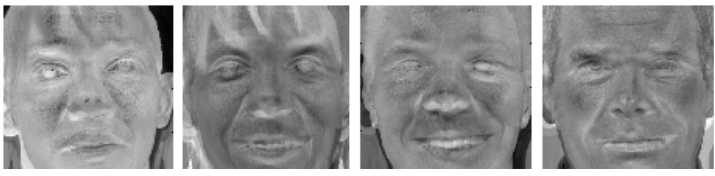
\includegraphics[width=7.15cm,height=2cm]{figuras/eigenfacesEx.png}
\label{fig:eigenfacesEx}
}
\subfigure[Exemplos de \textit{eigenpoints}]{
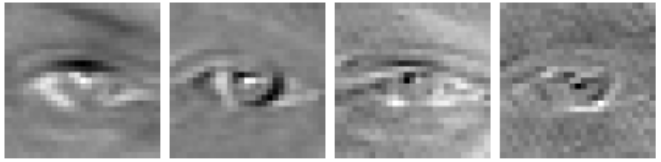
\includegraphics[width=7.15cm,height=2cm]{figuras/eigenPointsEx.png}
\label{fig:eigenpointsEx}}
\caption{Exemplos de \textit{eigenfaces}  � direita e a esquerda temos \textit{eigenpoints} extra�dos a partir de blocos centrados a partir do olho direito das imagens das faces.}
\end{figure}

\subsection*{Formula��o do IPD-B-PCA}

O m�todo proposto por Sabino \cite{waldir} consiste em aumentar a robustez dos filtros discriminativos atrav�s das componentes principais de maior energia, ou seja, cujos autovalores associados s�o maiores. Matematicamente podemos obter esses filtros da seguinte maneira: suponhamos uma  vari�vel aleat�ria que pode ser classificadas nas classes \{${\mathcal{A}_1},\,{\mathcal{A}_2},\,...,\,{\mathcal{A}_N}$\} onde: 

\begin{itemize}
\item A classe ${\mathcal{A}_1}$ ser� composta pela componente que desejamos detectar (${\mathcal{A}_1=\{\phi _i\}}$);

\item A classe ${\mathcal{A}_2}$ refere-se a deslocamentos lineares de $\phi _i$. A express�o $\phi _i^{n,m}$ relaciona o deslocamento linear da componente \textit{i} em \textit{n} \textit{pixels} na dire��o horizontal e \textit{m} na vertical. Considerando-se blocos quadrados de tamanho \textit{L} em que o centro do bloco cont�m o ponto fiducial de interesse, podemos escrever ${\mathcal{A}_2} = \{ \phi _i^{n,m}$, onde: $- L \le \,m,n\, \le \,L$, com $n,m \ne \,0\}$ .

\item A classe $\mathcal{B}$ ser� composta pelas demais componentes $\phi _j$, ou seja, as classes \{ ${\mathcal{A}_3},\,{\mathcal{A}_4},\,...,\,{\mathcal{A}_N}$\}.
\end{itemize}

Para projetarmos o nosso classificador utilizaremos a equa��o \eqref{vetorH_final}, levando-se em considera��o as premissas citadas teremos:

\begin{equation}\label{eq_ipd_pca}
{h_{{\phi _1}}} = {\left\{ {{p_1}{R_{A1}} + {p_2}{R_{A2}} + {p_B}{R_B}} \right\}^{ - 1}}\,{p_1}{R_{A1}}
\end{equation}

A Figura \ref{fig_ipd_pca} ilustra o esquema proposto, onde temos \textit{S} \textit{eigenpoints} ($\Phi  = \,{\phi _1},\,{\phi _2},\,...,\,{\phi _S}$), para cada um ser� projetado um filtro, de forma que estejam disposto do maior para o menor valor de vari�ncia (autovalores), desse modo, ${\lambda _1} > \,{\lambda _2} > ,...,\,{\lambda _S}$.

\begin{figure}[!htb]
\centering
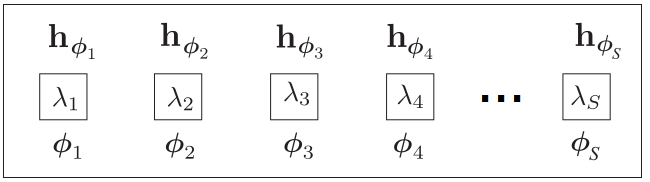
\includegraphics[scale=0.9]{figuras/esquema_Matriz.png}
\caption{\textit{S} classificadores para \textit{S} componentes principais.}
\label{fig_ipd_pca}
\end{figure}

Na Figura \ref{fig_schema}, podemos observar um \textit{eigenpoint} que refere-se ao olho direito considerando-se apenas a primeira componente principal. A componente $\phi_1$ foi calculada atrav�s de blocos de dimens�o 2L+1 (imagem mais � esquerda). Afim de obtermos a componente $\phi_2$ atrav�s de deslocamentos lineares at� o meio do bloco calculamos $\mathop {{\phi _i}}\limits^ \sim$ para blocos de dimens�o 4L+1 (imagem mais a direita). Assim, reescrevendo a Equa��o \eqref{eq_ipd_pca} em fun��o dessas pondera��es teremos:

\begin{figure}[!htb]
\centering
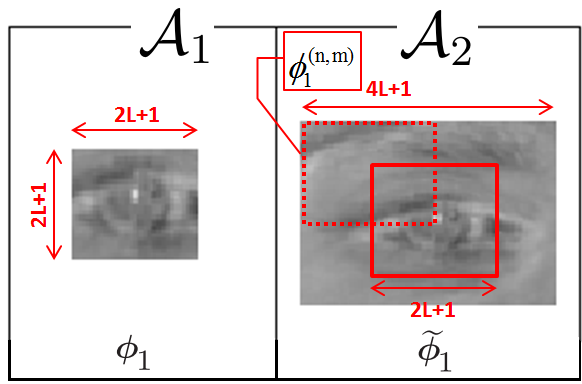
\includegraphics[scale=0.7]{figuras/Schema.png}
\caption{Desclocamento linear}
\label{fig_schema}
\end{figure}


\begin{equation} \label{eq_IPD-B-PCA_Final}
h{\phi _i} = {\left\{ \begin{array}{l}
{p_1}{\phi _i}{({\phi _i})^{T}} + {p_2}\frac{1}{{{{(2L + 1)}^2} - 1}}\,\sum\limits_{n =  - L\hfill\atop
n \ne 0\hfill}^L {\sum\limits_{m =  - L\hfill\atop
m \ne 0\hfill}^L {{\phi _i}^{(n,m)}({\phi _i}^{(n,m)})^{T} }} +\\
 + p(\mathcal{B})\,\frac{1}{{N - 1}}\,\sum\limits_{j = 1\hfill\atop
j \ne i\hfill}^N {{\phi _j}{{({\phi _j})}^{T}}} 
\end{array} \right\}^{ - 1}}\,{p_1}{\phi _i}
\end{equation}

Finalmente, a Equa��o \eqref{eq_IPD-B-PCA_Final} expressa o detector por produto interno utilizando an�lise de componentes principais. � interessante destacarmos que na constru��o dos padr�es de interesse da classe $\mathcal{A}_1$ podemos utilizar componentes levemente rotacionados ou deslocados, dessa forma � poss�vel construir detectores mais robustos. A classe ${\mathcal{A}_2}$ � de fundamental import�ncia, uma vez que se consider�ssemos somente as classes padr�es ($\mathcal{A}_1$) poder�amos incorrer em um poss�vel erro e detectar algo pr�ximo ao padr�o mesmo n�o sendo. Esse fato, deve-se a linearidade dos filtros, portanto, pequenas altera��es na entrada produzem apenas pequenas perturba��es na sa�da. Assim, a adi��o da classe ${\mathcal{A}_2}$ permite ao classificador rejeitar pequenos deslocamentos lineares de forma mais precisa e com uma maior efici�ncia.
                      
\section{Computa��o Paralela}

Com o desenvolvimento da inform�tica em diversos campos houve uma exig�ncia por um maior poder de processamento por parte dos programas. \textit{Softwares} tornaram-se mais sofisticados e computacionalmente mais pesados, assim os processadores come�aram a ficar obsoletos face � essa excesso de demanda por processamento. A solu��o encontrada no in�cio foi acelerar o rel�gio do processador, por�m, com essa acelera��o apareceu o problema do superaquecimento desses chips. A solu��o para esse problema veio com a adi��o de mais de um n�cleo no mesmo \textit{chip}, atrav�s da tecnologia \textit{multicore}. Dessa forma, eliminaria-se a necessidade de cada n�cleo trabalhar em frequ�ncias muito elevadas, tendo somente como base um esquema de escalonamento de tarefas mais eficiente \cite{tanenbaum2013sistemas}.

A ideia desse paradigma de programa��o � "quebrar" o programa em v�rias partes e process�-los de forma concorrente (paralela), ganhando assim tempo na execu��o da tarefa. � interessante notarmos que nem todas as partes de um programa s�o "paraleliz�veis", portanto para esse tipo de aplica��o a exist�ncia de um ou mais n�cleos n�o resultar� na celeridade de sua execu��o. O paralelismo pode ser expl�cito quando o pr�prio programador controla a concorr�ncia ou impl�cito, quando cabe ao compilador do sistema realizar o paralelismo.

Existem diversos tipos de paralelismo, podermos destacar: 

\begin{itemize}
\item \textbf{No bit}: Nesse tipo dobrava-se o tamanho da palavra (unidade de informa��o utilizada para cada tipo de computador), com isso dobrava-se a quantidade de processamento por ciclo e consequentemente a diminui��o da quantidade de instru��es \cite{sriram2009embedded};

\item \textbf{Na instru��o}: Assumindo que um programa de computador � constitu�do por um conjunto de instru��es interpretados pelo processador, pode-se combinar essas instru��es em blocos que podem ser executados de forma concorrente sem alterar o resultado final\cite{sriram2009embedded};

\item \textbf{No dado}: Geralmente ocorre em la�os (\textit{loops}), nas quais uma intera��o depende de outros resultados\cite{sriram2009embedded};

\item \textbf{No tarefa}: � inerente as aplica��es (programas), caracteriza-se ao oposto do paralelismo em dados, ou seja, diferentes c�lculos podem ser realizados no mesmo ou em diferentes tipos de dados\cite{sriram2009embedded};

Um ponto crucial para se obter um alto desempenho na computa��o paralela tange no que diz respeito ao acesso da mem�ria. Existem duas arquiteturas quanto as formas de acesso a mem�ria:

\item \textbf{Centralized Multiprocessor ou Uniform Memory Access Multiprocessor (UMA)}: Nesse modelo as tarefas compartilham de um mesmo espa�o de mem�ria e a comunica��o � mais simples, pois utiliza-se de uma �rea comum na mem�ria (Figura \ref{fig_Compartilhada} a);

\item \textbf{Distributed Multiprocessor ou Nonuniform Memory Access Multiprocessor (NUMA)}: Nesse padr�o cada processador possui o seu pr�prio endere�o na mem�ria. A comunica��o entre esses processadores � feito atrav�s de mensagens (Figura \ref{fig_Ditribuida} b). {\color{red} Eu vou concatenar as duas Figuras em uma s�. S� n�o fiz porque ainda n�o acertei como se faz})
\end{itemize}

\begin{figure}[h]
\center
\subfigure[Mem�rica compartilhada - UMA]{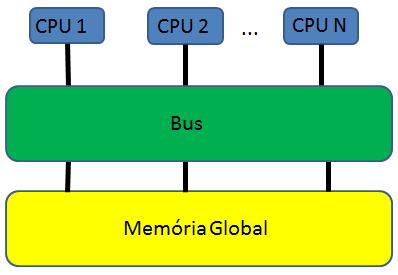
\includegraphics[width=7cm]{figuras/Tipos_Memorias_Shared.PNG}}\label{fig_Compartilhada}
\qquad
\subfigure[Mem�rica compartilhada - NUMA]{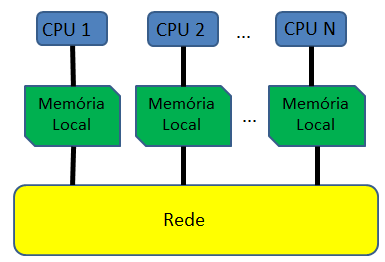
\includegraphics[width=7cm]{figuras/Tipos_Memorias.PNG}}
\caption{Arquiteturas de computa��o paralela a) Mem�ria compartilhada e b) mem�ria distribu�da.}\label{fig_Ditribuida}
\end{figure}


\subsection{OpenMP}

Quanto ao paralelismo, podemos destacar duas formas: o paralelismo expl�cito e o paralelismo impl�cito. A seguir destacamos algumas caracter�sticas de cada uma:

\begin{itemize}
\item \textbf{paralelismo expl�cito}:

\item \textbf{paralelismo impl�cito}:

\end{itemize}


\subsection{M�tricas de desempenho na Computa��o Paralela}

{\color{red} A id�ia aqui aqui � apresentar o/os m�todos mai utilizados na avalia��o de desempenho quando comparados com a programa��o sequencial.}






  %
\chapter{Sistema de Detec��o de Pontos Fiduciais utilizando Classificadores C-SVC}\label{cap-sistema1}

%\textcolor{red}{Neste cap�tulo s�o apresentadas as contribui��es deste trabalho e a descri��o do sistema de detec��o de pontos fiduciais utilizando classificadores lineares C-SVC. Na Se��o \ref{sec:bloco_negativo} s�o apresentadas as contribui��es cient�ficas que justificam a realiza��o desta pesquisa. A seguir, apresentamos o sistema de detec��o de pontos fiduciais, divido em duas etapas: treinamento e teste. A etapa de treinamento, por sua vez � dividida em Pr�-processamento, Modelo Gaussiano � Priori, \emph{Salt and Pepper}, Transforma��o Matriz-Vetor e Treino do Classificador C-SVC. A etapa de teste, por sua vez apresenta as etapas de Pr�-processamento, Modelo Gaussiano � Priori, Transforma��o Matriz-Vetor e Classifica��o do C-SVC.}



\section{Sistema de Detec��o de Pontos Fiduciais utilizando Classificadores SVM}\label{sec:sistema}

%revis�o-final - waldir 20/01/2014

Pontos fiduciais podem ser definidos como marca��es de refer�ncia \cite{viola-jones2,pontos-fiduciais1, pontos-fiduciais2, pontos-fiduciais3}. Em algumas aplica��es/problemas \cite{fundamentos1, fundamentos2} a detec��o de pontos fiduciais � uma etapa importante. Por exemplo, nos sistemas apresentados em  \cite{fundamentos1, fundamentos2} que abordam o problema do reconhecimento de express�es faciais e estima��o de pose os autores utilizam a detec��o de pontos fiduciais para compor o sistema completo. Nestes sistemas, a detec��o de pontos fiduciais � feita para mapear pontos ao redor de uma regi�o da face, como por exemplo, a boca e em seguida, o mapeamento � utilizado para integrar um modelo de forma culminando no reconhecimento da express�o da boca e estima��o da pose da face.


  %\chapter{Experimentos e Resultados}\label{cap-experimentos}

\section{Base de Dados}

%A base de dados � um elemento essencial para o procedimento de experimentos deste sistema de detec��o de pontos fiduciais pois disponibiliza as imagens utilizadas no procedimento de treino e teste. A base de dados auxilia o sistema de detec��o de pontos fiduciais nas caracter�sticas para o treino do algoritmo SVM e ao final para a extra��o de caracter�sticas para no c�lculo do desempenho do sistema de detec��o de pontos fiduciais. Assim, de acordo com a base de dados, podemos identificar se o sistema de pontos fiduciais desenvolvido � robusto.

Nesta disserta��o, iremos utilizar duas bases de dados denominadas por \emph{BioID} e \emph{Feret}. A \emph{BioID} � uma base de dados caracterizada por apresentar varia��es da pose, condi��es de ilumina��o natural e  \emph{backgrounds} distintos. Estas caracter�sticas tornaram a \emph{BioID} uma base de dados amplamente utilizada em pesquisas para a compara��o de desempenho entre t�cnicas de classifica��o aplicadas � sistemas de detec��o de pontos fiduciais. A base de dados \emph{BioID} original � composta por $1521$ imagens em escala de cinza com resolu��o de $384 \times 286$. A \emph{BioID} possui imagens que foram retiradas de $23$ indiv�duos em diferentes formas. Neste conjunto, os indiv�duos podem conter �culos, barba e bigode. Al�m das imagens, a base de dados possui uma anota��o de $20$ pontos na face e outra contendo somente os olhos. Na Figura \ref{fig20}, podemos visualizar exemplos das imagens da base de dados \emph{BioID}.

%[width=8cm]
\begin{figure}[!htb]
  % Requires \usepackage{graphicx}
  \centering
  \includegraphics[scale=0.8]{bioid.eps}
  \caption[Exemplos de imagens da base dados \emph{BioID}.]{Exemplos de imagens da base dados \emph{BioID} \cite{bioID}.}
  \label{fig20}
\end{figure}


  %\chapter{Conclus�o}\label{cap-conclusao}

\hyphenation{ge-ne-ra-li-za-��o} \hyphenation{ma-te-m�-ti-ca} \hyphenation{pro-ble-ma}
\hyphenation{e-fe-tu-ar-mos} \hyphenation{ne-ces-s�-rio}

%\section{Considera��es Finais da Disserta��o}

Nesta disserta��o, investigamos os par�metros que influenciam na gera��o do hiperplano �timo respons�vel pela separa��o dos dados das classes de positivos e negativos da t�cnica SVM.
%%%%%%%%%%%%%%%%%%%%%%%%%%%%%%%%%%%%%%%%%%%%%%%%%%%%%%%%%%




%%%%%%%%%%%%%%%%%%%%%%%%%%%%%%%%%%%%%%%%%%%%%%%%%%%%%%%%%%
%% Referencias
  \backmatter
  \nocite{*}
  \bibliographystyle{cls_bst/bst_ufam}
  \bibliography{capitulos/referencias}
%%%%%%%%%%%%%%%%%%%%%%%%%%%%%%%%%%%%%%%%%%%%%%%%%%%%%%%%%%




%%%%%%%%%%%%%%%%%%%%%%%%%%%%%%%%%%%%%%%%%%%%%%%%%%%%%%%%%%
%% ap�ndice
  \appendix
 % \chapter{Artigos Publicados}\label{apendice}

Neste ap�ndice, apresentamos os artigos desenvolvidos nesta Disserta��o.

\section{Artigos Diretamente Relacionados ao Tema}
\begin{enumerate}
  \item SILVA, L. E. S.; SANTOS, K. V.; SILVA JUNIOR, W. S. "Sistema de Detec��o de Pontos Fiduciais utilizando Classificadores Lineares C-SVC". In: {\it Anais do XXXI Simp�sio Brasileiro de Telecomunica��es}, Setembro de 2013, Fortaleza. SBrT'13, 2013.
\end{enumerate}

\begin{enumerate}
  \item SILVA, L. E. S.; SANTOS, K. V.; TOMAZ JUNIOR, P. D.; SILVA JUNIOR, W. S. "Fiducial Points Detection Using SVM Linear Classifiers". In: {\it Second International Conference on Computacional Science and Engineering}, Dubai, 2014.
\end{enumerate}

\section{Outros Artigos}
\begin{enumerate}
  \item SANTOS, K. V.; SILVA, L. E. S.; SILVA JUNIOR, W. S. "Avalia��o do Desempenho dos Filtros Discriminativos em um Sistema de Detec��o de Pontos Fiduciais". In: {\it Anais do XXXI Simp�sio Brasileiro de Telecomunica��es}, Setembro de 2013, Fortaleza. SBrT'13, 2013.
\end{enumerate}

\begin{enumerate}
  \item SILVA, L. E. S.; SANTOS, K. V.; SILVA JUNIOR, W. S. "Fiducial Points Influence of Quantity of Principal Component In Discriminative Filtering". In: Second International Conference on Computacional Science and Engineering, Dubai, 2014.
\end{enumerate} 
 %\input{capitulos/apendice3}
%%%%%%%%%%%%%%%%%%%%%%%%%%%%%%%%%%%%%%%%%%%%%%%%%%%%%%%%%%



\end{document}
